%%%%%%%%%%%%%%%%%%%%%%%%%%%%%%%%%%%%%%%%%%%%%%%%%%%%%%%%%%%%%%%%%%%%%%%%%%%%%%%%%%%%%%%%%%%%%%%%%%%%%%
%
%   Filename    : chapter_5.tex 
%
%   Description : This file will contain details regarding the crowdsourcing platform.
%                 
%%%%%%%%%%%%%%%%%%%%%%%%%%%%%%%%%%%%%%%%%%%%%%%%%%%%%%%%%%%%%%%%%%%%%%%%%%%%%%%%%%%%%%%%%%%%%%%%%%%%%%
\chapter{WeCyclePH}

WeCyclePH is a crowdsourcing platform and mobile application designed to capture cyclists' real-world experiences by collecting GPS data, optional video recordings, user annotations, and feedback. By supporting data collection across varied urban environments, the platform enables the generation of a rich dataset that combines spatial, contextual, and user-contributed data. This data supports research into urban cycling conditions and infrastructure planning and powers an open-access public map.

\section{Design Refinements Through Iterative Testing}

The evolution of the WeCyclePH mobile application was guided by an iterative development process that combined real-world testing, structured evaluation, and targeted design refinements. From its earliest conception, the platform was envisioned as a tool for cyclists to log rides, annotate infrastructure conditions, and contribute to a collective dataset for research and advocacy. However, the form this tool ultimately took was shaped as much by the realities of cyclist behavior and technological constraints as by the original design vision.

Each iteration, from the initial prototype through to the public beta, was informed by a cycle of implementation, field testing, and feedback analysis. Across these phases, the application shifted from a video-centric annotation system with rigid onboarding requirements to a more flexible, GPS-based reporting platform with streamlined contribution flows and privacy controls. This transformation was neither linear nor cosmetic; it reflected a fundamental rethinking of what it meant to make crowdsourced data collection accessible, sustainable, and safe for cyclists in diverse contexts.


\subsection{Initial Design Assumptions}

The earliest design of WeCyclePH was built upon a set of core assumptions about how cyclists would engage with a data collection platform. Foremost among these was the expectation that contributors would be both willing and technically able to record their entire rides in video form and later upload this footage in its entirety. This approach was intended to provide rich contextual information for annotations, ensuring that each reported hazard, infrastructure feature, or experiential note was anchored to a verifiable visual record.

It was further assumed that cyclists would be comfortable navigating post-ride annotation workflows modeled after familiar media editing interfaces. The design drew heavily on paradigms from consumer-facing tools such as Strava, which popularized streamlined ride logging and performance tracking, and CapCut or similar timeline-based video editing platforms, which allowed precise placement of markers or clips along a chronological sequence. By adapting these paradigms, the prototype aimed to make the annotation process both familiar and precise: a cyclist could scrub through the video timeline, locate the exact moment a hazard occurred, and attach a structured annotation tied to that timestamp.
The feature set of the initial prototype reflected these priorities:

\begin{itemize}
    \item Ride Recording: GPS-enabled ride tracking, intended to synchronize spatial data with video footage.
    \item Full-Ride Video Uploads: The central contribution method, allowing comprehensive review and precise annotation.
    \item Video-Based Annotation Tool: A timeline interface where users could insert annotations at specific temporal points in the video.
    \item Ride History: An archive of past rides, accessible for review or further annotation.
    \item Media Management: Upload and storage of ride videos, with the potential for future image support.
    \item Profile Section: Basic user account management, including personal details and ride statistics.
    \item Login and Registration: A standard account creation process, including email verification for authentication.
\end{itemize}



While the design promised highly detailed and verifiable cycling data, it also imposed significant demands on contributors. Uploading entire ride videos could be time-consuming, particularly in areas with limited bandwidth. The requirement to review the entire recording before annotating introduced additional cognitive and time costs, which risked deterring casual contributors. Moreover, by centering the annotation process exclusively around video, the system assumed that every contributor had the necessary storage capacity, camera hardware, and willingness to capture long-duration footage. This assumption that would later prove to be a critical friction point in user adoption.

\begin{figure}[H]
\centering
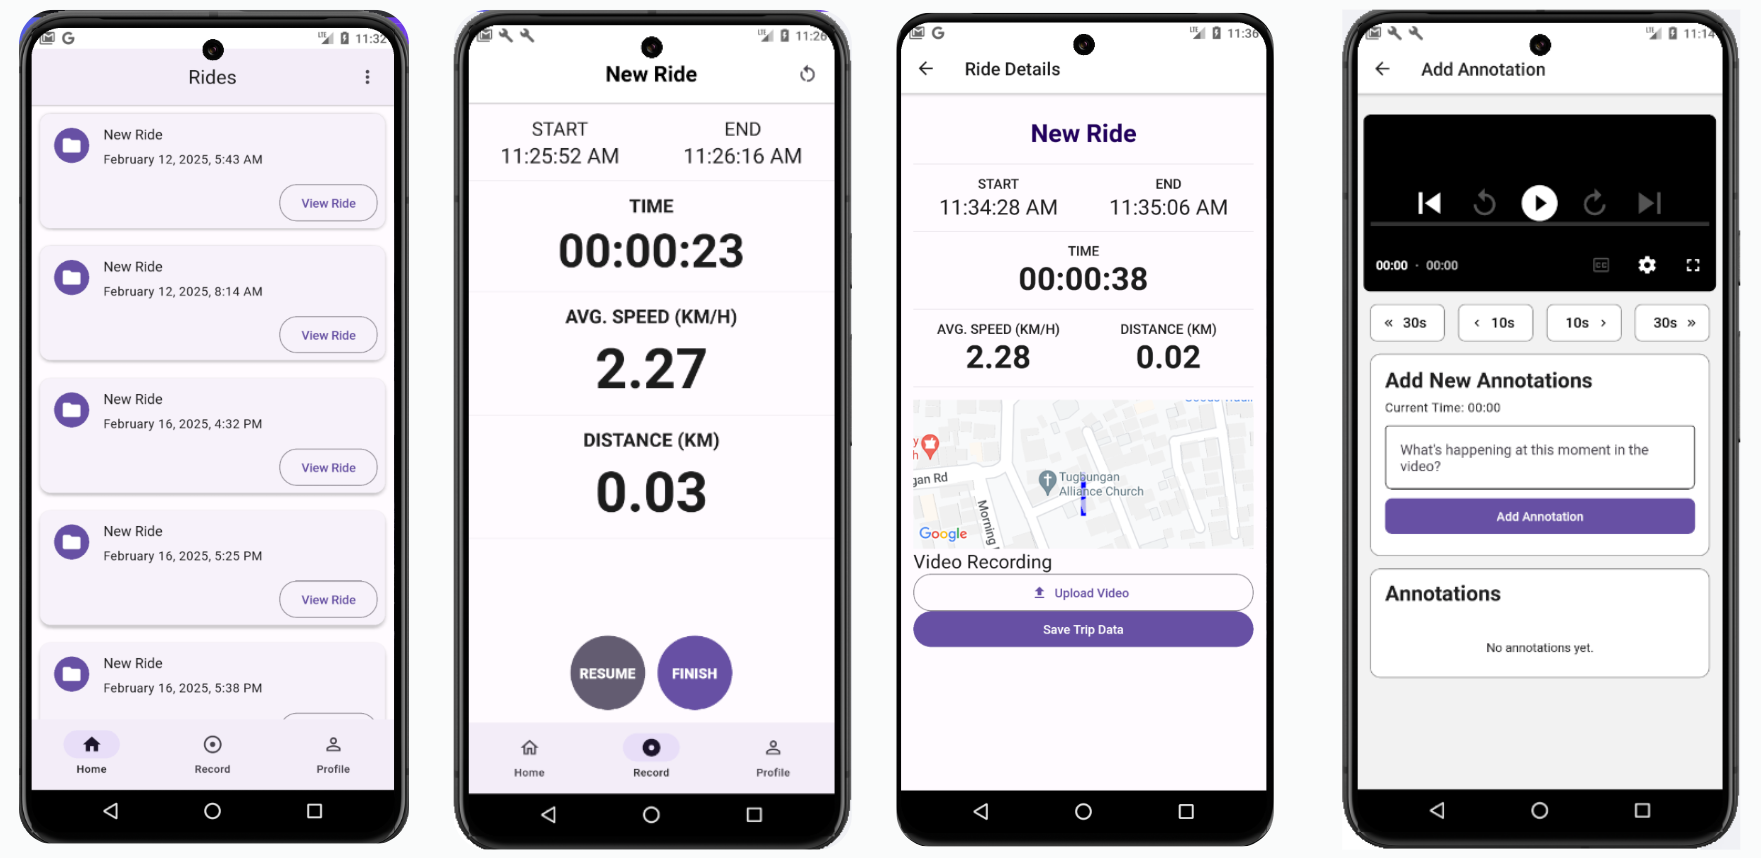
\includegraphics[width=0.9\linewidth]{figures/chapt5/initialVersionPreview.png}
\caption{In-app screenshots of the initial WeCyclePH prototype, showcasing core features such as ride recording, annotation tools, and media upload options.}
\label{fig:initialVersionPreview}
\end{figure}

\subsection{First Validation: Guerilla Testing}

The first phase of validation for WeCyclePH was conducted through guerrilla testing, aimed at assessing the app's initial usability and gauging user understanding of its core features. This phase involved casual cyclists and first-time users interacting with the prototype in real-world settings, allowing the team to observe natural behavior and friction points during actual usage. Rather than structured evaluations, the goal was to capture spontaneous reactions and feedback from participants with varying levels of tech familiarity and cycling experience. Through this process, the team was able to surface early pain points, interface confusion, and performance bottlenecks, which would go on to shape the next iteration of the application.

\begin{figure}[H]
\centering
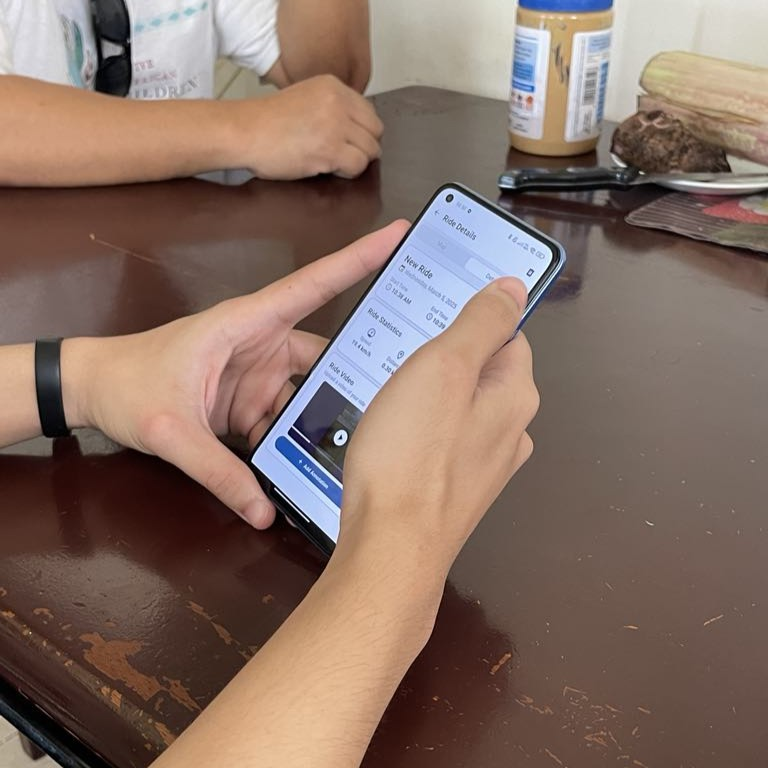
\includegraphics[width=0.6\linewidth]{figures/chapt5/guerillatesting.jpg}
\caption{Participant testing the initial WeCyclePH app design during guerrilla testing, demonstrating early user interaction with the platform’s core features.}
\label{fig:GuerillaTestingPicture}
\end{figure}

\subsubsection{Key Findings}

Based on the guerrilla testing, several key issues were identified, reflecting initial usability concerns and user preferences.

One prominent issue was the friction experienced during account creation. Several users expressed frustration over the strict password requirements and email verification processes, particularly those who self-identified as non-tech-savvy. They advocated for a simplified sign-up flow that lowers the barrier to entry, especially for casual or older cyclists who may not be familiar with stringent security standards.

The user interface (UI) was largely seen as functional, yet incomplete. While some praised its simplicity, others pointed out elements that felt redundant or lacking polish. The Home button, for instance, was considered unnecessary due to existing navigation options, and the excessive spacing in the top bar and general layout was noted. The Edit Profile page was highlighted by multiple users as particularly underdeveloped, slow to load and offering limited customization. Suggestions included the ability to change one's name, email, or profile picture, as well as the addition of a delete account option for privacy-conscious users.

When it came to the core feature of ride recording, participants responded positively to the streamlined Record button. Regular cyclists appreciated how effortless it was to start tracking rides. However, less frequent users were puzzled by metric outputs (e.g., speed, distance), particularly when unsupported by contextual map data. One suggestion involved integrating a live map view during rides to help users better understand their location and performance metrics.

Annotation functionality was one of the most criticized aspects. Multiple users encountered problems saving annotations or found the process too slow, with delays ranging from 30 seconds to over a minute. Several proposed adding a dedicated “Add Annotation” button during the ride session for quick and accurate data input when encountering hazards. Users also wanted annotations to be visible on the map afterward, emphasizing both the utility of location-based context and the frustration when contributions appeared to vanish or lacked feedback.

Feature discoverability presented another barrier. Participants noted confusion in locating actions such as deleting rides, editing trip titles, or changing profile settings. A lack of in-app guidance or tooltips was especially detrimental for first-time users. Suggestions included implementing onboarding tutorials or rethinking page layouts, such as turning the profile page into a sidebar to improve navigability.

Performance concerns were widespread. Slow app response times, especially when saving annotations or loading profile pages, affected user experience. Bugs were observed when recording longer sessions, and some noted disappearing navigation elements after actions like editing. Despite these setbacks, the app's core functionality generally worked as intended, with many users acknowledging its potential.

\subsubsection{Implications for Application Development}
The feedback from guerrilla testing revealed several areas for improvement in the app. Firstly, simplifying navigation was critical, including removing redundant UI designs, buttons, and streamlining the profile editing process. Secondly, integrating a real-time map for route tracking was necessary to meet cyclists' needs for visualizing their cycling path and progress. Lastly, streamlining the onboarding process to reduce friction for user acquisition.

These findings served as the foundation for the next iteration of the app, which was tested in the Closed Beta Testing phase.


\subsection{Closed Beta}

The feedback collected during guerrilla testing directly informed a series of key design refinements that shaped the Closed Beta of WeCyclePH. In response to early usability concerns, we prioritized lowering entry barriers, improving feature discoverability, and enhancing real-time feedback during rides. These changes laid the groundwork for a more polished and accessible experience, ready to be validated in broader, real-world use.

\begin{figure}[H]
\centering
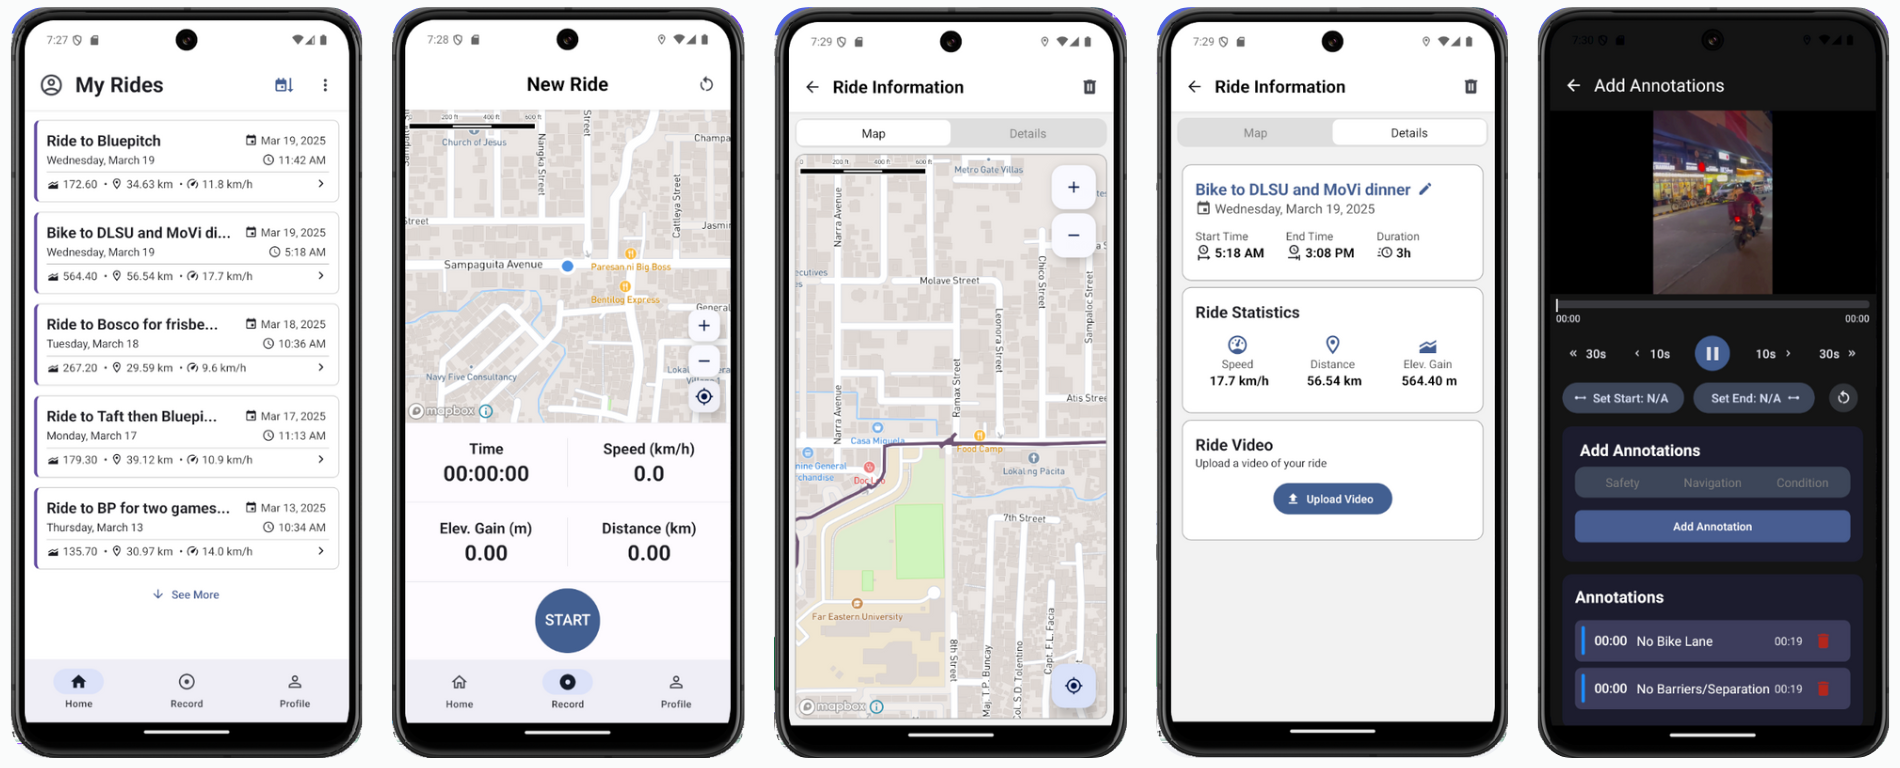
\includegraphics[width=0.9\linewidth]{figures/chapt5/closedBetaPreview.png}
\caption{In-app screenshots of the closed beta version of WeCyclePH, highlighting refined core features and interface improvements implemented in response to guerrilla testing feedback.}
\label{fig:closedBetaPreview}
\end{figure}

To streamline the onboarding experience, the registration process was restructured. Participants had previously voiced frustrations with the app's strict password requirements and email verification steps. In response, the verification process was deferred, allowing users to register and access the app immediately, with email confirmation requested only after account creation. Password criteria were also revised to be more user-friendly while still maintaining security standards.

Navigation and discoverability were addressed through targeted UI changes. Users can now create multiple rides with the same name, improving flexibility and organization for frequent riders. The home screen and profile page layouts were cleaned up, while the profile editor was revamped for improved performance and simpler flow.

Significant effort was made to enhance real-time location awareness. A live GPS map was integrated into the ride recording screen, providing users with spatial feedback and supporting a better understanding of their current location and ride progress, an issue highlighted during the guerilla tests. This also improved the interpretability of performance metrics like distance and speed, especially for less experienced users.

These adjustments formed the basis for the Closed Beta Testing, which was deployed to a group of testers for real-world validation. The application was distributed via direct APK download through Google Drive, with testing conducted by experienced cyclists in a controlled environment. This phase aimed to evaluate the system's stability, media handling flow, and user comprehension of the application under authentic cycling conditions, bridging the gap between initial prototyping and a more dynamic usage scenarios.

\begin{figure}[!h]
    \centering
    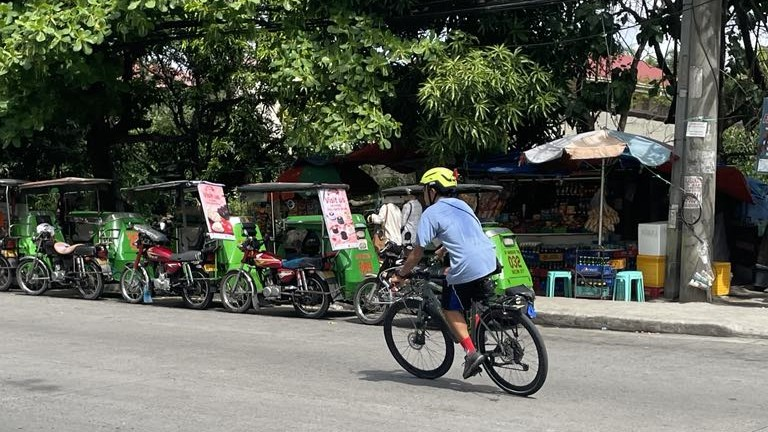
\includegraphics[width=1\linewidth]{figures/chapt5/closedbetatest.jpg}
    \caption{Participant using the WeCyclePH application during closed beta testing, conducted with experienced cyclists to evaluate system stability, media handling, and user comprehension in real-world cycling conditions.}
    \label{fig:ClosedBetaPicture}
\end{figure}

\subsubsection{Key Findings}
During the Closed Beta Testing phase, several significant challenges were identified, particularly related to the app's video upload process, map features, privacy concerns, and performance. These findings provided crucial insights that guided the development of the app.

One of the main issues faced by participants was the difficulty with full-video uploads. Participants found the process of uploading entire cycling session videos to be impractical and time-consuming, especially when riding in areas with limited data connectivity or time constraints. As CB02 shared, \textit{“Uploading the entire video was too much... I prefer short clips that I can easily send, especially if I'm riding in traffic.”} Similarly, CB03 echoed this sentiment, stating, \textit{“I can upload short clips, yeah, but a full ride? That's a little bit too heavy.”} This feedback made it clear that the app's current upload system was not feasible for regular cycling use. Participants recommended switching to shorter video clips and integrating an auto-capture functionality that would automatically record important moments during the ride, such as accidents or near-misses, without interrupting the cycling experience. CB02 suggested, \textit{“What if it's like Waze, wherein you just press the button to report that something happened, and it takes the last 10 seconds of where you were and labels it?”}

Another key finding was the desire for enhanced map features and better ride tracking. Participants expressed a strong preference for real-time route tracking and the ability to visualize their cycling routes as they rode. CB02 commented, \textit{“I like having a map, but the app didn't show me where I was. I had to guess.”} CB01 further emphasized the importance of local route data, stating, \textit{“It's more of the existing data near their place where they usually bike to, that gives them motivation to use the app.”} Users also wanted the ability to view their ride history and monitor performance metrics such as distance, speed, and duration. CB02 noted, \textit{“One of the things when I finish a ride, I love to see the stats of my ride, that's why I like the auto pause, because it doesn't mess up my stats.”}

Privacy concerns were also raised regarding the sharing of accident footage. Participants felt uncomfortable with the idea of their incident videos being shared publicly. As CB01 expressed, \textit{“Yeah, I don't want to share accident footage publicly; that feels too invasive.”} CB03 added a nuanced view, stating, \textit{“I don't mind recording, but if it's something serious like a near miss or crash, I want control over who sees it. It feels a little bit uncomfortable to post something like that, but I do see the vision why it's important.”} To address this, participants recommended adding a private incident-reporting feature, where users could send footage directly to app administrators or emergency services without sharing it publicly. Implementing such a feature would alleviate privacy concerns while maintaining the app's utility in critical situations.

The incident reporting system also received feedback about being too cumbersome. Participants felt that the current process, which required manual annotations in video footage, was too labor-intensive and suggested that incidents should be flagged automatically or through a quick-report directly via the GPS map. CB02 emphasized, \textit{“It was too much effort to manually annotate my rides in videos. I'd prefer if I can report quickly and go on about my ride.”} Similarly, CB03 recommended automation support: \textit{“If it could auto-tag based on my footage, even just suggest timestamps where the road shook or I slowed down, that would save a lot of effort.”} This feedback highlighted the need to automate or simplify the incident reporting process, making it quicker and easier for cyclists to document safety concerns during their rides.

\subsubsection{Implications for Application Development}
The findings from Beta Testing emphasized the need for several improvements and major feature rebuild to enhance the app's usability, performance, and privacy controls. These improvements addressed the concerns raised during testing, setting the stage for the next phase of development as the app moves into public-beta deployment.

\subsection{Final Design Considerations Towards Public Beta}

The final version of WeCyclePH integrated major design overhauls in response to the persistent issues identified during closed beta testing. These adjustments were geared toward lowering contribution friction, improving feature clarity, and supporting real-world cycling behaviors. Rather than layering in new features, the focus was on rebuilding existing systems in a way that was simpler, safer, and more intuitive for everyday use.

\begin{figure}[H]
\centering
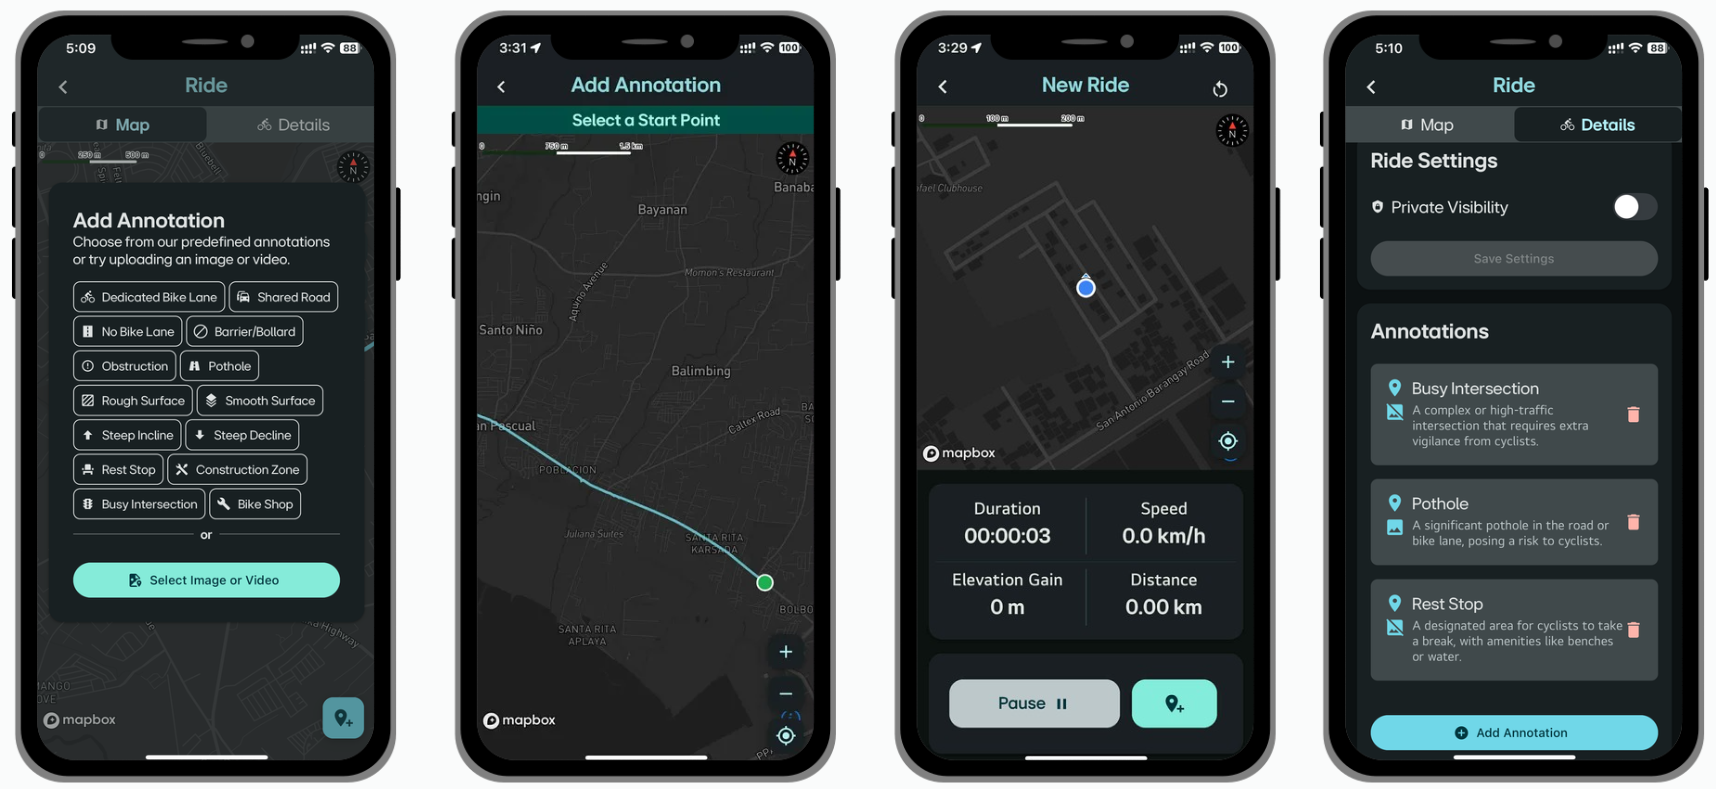
\includegraphics[width=0.9\linewidth]{figures/chapt5/publicBetaPreview.png}
\caption{In-app screenshots of the public beta release of WeCyclePH, showcasing redesigned core features aimed at reducing contribution friction, improving clarity, and supporting safer, more intuitive real-world cycling use.}
\label{fig:publicBetaPreview}
\end{figure}

\paragraph{Annotation Feature Rebuild}
 
 One of the most significant shifts was the complete redesign of the annotation feature. Users now annotate directly on the GPS map, removing the dependency on uploading ride videos before contributing. This change eliminated a major bottleneck in the contribution process and allowed annotations to happen independently of video footage.

 In parallel, a Quick Report button was introduced, allowing users to tag road hazards in real time with a single tap while riding. This feature was made possible by the transition to GPS-based annotations, which removed the need for video timestamps during contribution.
 
To further reduce cognitive load, a set of predefined annotation classes was also implemented. These classes simplify reporting, enabling users to select from a list of common road issues (e.g., potholes, blocked bike lanes) rather than writing freeform text. These enhancements combined to make annotations faster, easier, and more accessible, especially during active commutes.

\paragraph{Media Contribution Redesign}

The media upload process was restructured to reduce the burden of uploading long, high-resolution videos. The system now supports short video clips, which are automatically matched to ride data using date-time metadata. In addition, users can now upload photos alongside their annotations to provide visual context without requiring full video footage.

While full-ride video uploads remain supported for advanced users or those with external cameras, they are no longer a prerequisite for contributing. This shift made the platform more inclusive to cyclists using basic smartphones or those with limited connectivity.

\paragraph{Improved Interface and Flow}

To improve navigational clarity, several refinements were made to the app's interface and ride flow. Visual elements were streamlined to make key actions such as uploading images, reviewing rides, or editing details more visible and easier to access. These small but important changes enhanced the overall usability of the app, particularly for first-time users.

\paragraph{Privacy Controls}

Finally, in response to concerns raised during closed beta, granular privacy settings were introduced for all uploaded media. Users now have the option to label content as public, private, or admin-only, giving them full control over how sensitive data such as crash footage or near-miss incidents is shared. This ensures contributors feel safe and respected while still allowing the platform to surface important safety data when needed.


% \subsection{Reflections on the Iterative Process}

% The transition from a video-centric annotation model to a GPS-based quick-report system reflected a deepened understanding of user context: cyclists often ride in environments where connectivity is limited, safety is paramount, and time for post-processing is scarce. Iterative testing ensured that each design shift was grounded in observed behavior rather than theoretical assumptions.

% \begin{table}[H]
% \centering
% \label{tab:iterative_changes}
% \begin{tabular}{|p{2.5cm}|p{5cm}|p{5cm}|}
% \hline
% \textbf{Testing Phase} & \textbf{Key User Concern} & \textbf{Design Change} \\ \hline
% Guerrilla & Hidden delete/upload options & UI rework for discoverability \\ \hline
% Guerrilla & Lack of live map view & Added GPS map integration \\ \hline
% Closed Beta & Full-video uploads too heavy & Short clip \& photo support \\ \hline
% Closed Beta & Manual annotation too slow & Quick Report + GPS-based tagging \\ \hline
% Closed Beta & Confusing post-ride flow & Post-ride annotation prompts \\ \hline
% Closed Beta & Privacy concerns with media & Granular privacy settings \\ \hline
% \end{tabular}'
% \caption{Summary of key user concerns identified during guerrilla and closed beta testing of WeCyclePH, and the corresponding design changes such as adding GPS map integration, quick reporting, and granular privacy settings that shaped the platform into a user-informed, real-world-ready tool by the public beta launch.}
% \end{table}

% This journey underscored the importance of embedding testing into every stage of development. By the time the public beta launched, \textit{WeCyclePH} was no longer just an experimental prototype, it was a platform informed by real-world cycling experiences, tailored to the realities of contributor behavior, and ready for deployment at scale.

\section{System Architecture}
The platform follows a modular client-server architecture consisting of a React Native mobile application, a web-based visualization dashboard, and a Firebase-powered backend. The mobile client facilitates data capture, while the backend manages secure storage and synchronization. This modular design ensures scalability and adaptability as user participation increases.

Data flow begins with users initiating trip recordings via the mobile app, during which GPS logs and optional media are captured. These are uploaded to Firebase, where they are organized under each user profile. A custom backend infrastructure stores this data and enables further downstream processing for visualization and research. Figure~\ref{fig:data_flow} illustrates the overall data flow through the platform.

\begin{figure}[H]
\centering
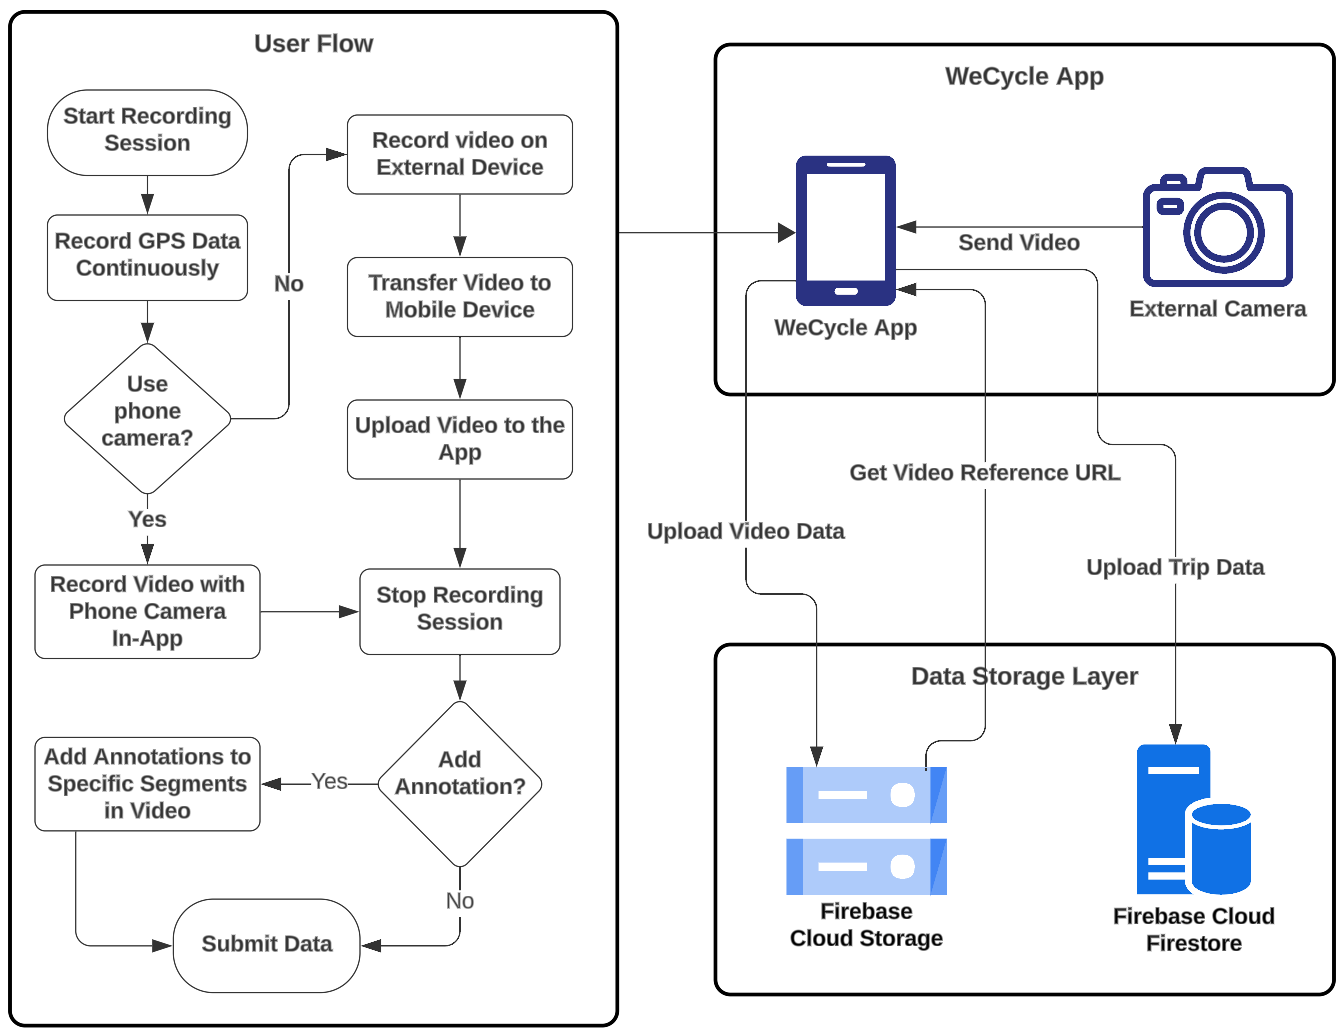
\includegraphics[width=1\linewidth]{figures/data_flow.png}
% \caption{Diagram of the user data flow throughout the system from the user's device to the cloud database and storage}
\caption{Diagram illustrating the end-to-end user data flow in WeCyclePH, from trip recording and media capture on the mobile app to secure storage, synchronization, and processing in the cloud backend for visualization and research.}
\label{fig:data_flow}
\end{figure}

The Firestore NoSQL database is structured as a nested collection-document hierarchy. Each ride is a document within the \texttt{rides} collection and contains both a \texttt{map} subcollection (with a single \texttt{points} document) and an \texttt{annotations} subcollection. A separate \texttt{users} collection holds user account metadata, though it is not the focus of our work. This hierarchical design enables efficient retrieval of ride-level metadata, GPS traces, and user-generated annotations, as shown in Figure~\ref{fig:firestore_schema_text}.

\begin{figure}[H]
\centering
\begin{lstlisting}[basicstyle=\ttfamily\footnotesize, frame=single]
rides (collection)
|-- {rideId} (document)
    |-- rideName: string
    |-- startTime: number (epoch ms)
    |-- endTime: number
    |-- duration: number (seconds)
    |-- distance: number (meters)
    |-- averageSpeed: number (m/s)
    |-- elevationGain: number (meters)
    |-- userId: string
    |-- map (subcollection)
    |   |-- points (document)
    |       |-- items: array of GPS points
    |           |-- coordinate: { 
                        latitude: number, 
                        longitude: number 
                    }
    |           |-- timestamp: number
    |           |-- elevation: number (optional)
    |-- annotations (subcollection)
        |-- {annotationId} (document)
            |-- id: string
            |-- rideId: string
            |-- userId: string
            |-- mediaUri: string (optional)
            |-- mediaType: string (optional)
            |-- points: array of RidePoint
            |-- sentiment: string (optional)
            |-- annotationLabel: string
            |-- type: "point" | "segment"
            |-- additionalTags: array of string (optional)
            |-- createdAt: number

users (collection)
|-- {userId} (document)
    |-- username: string
    |-- createdAt: number (epoch ms)
    |-- email: string
\end{lstlisting}
\caption{Text-based representation of the Firestore collection and document schema used in WeCyclePH}
\label{fig:firestore_schema_text}
\end{figure}




\section{Platform Components}
\subsection{Front-End}
The front-end of the application was developed using React Native with the Expo framework. React Native is a popular open-source framework that allows developers to build native mobile applications using JavaScript/TypeScript and React. This framework enables the creation of cross-platform apps that function seamlessly on both iOS and Android devices using a single codebase. Expo enhances the development process by providing a suite of tools and services that simplify development, building, and deployment.

Key features of the app include real-time GPS tracking and optional video recording functionality, all presented through a user-friendly interface. The user interface is designed with accessibility in mind, offering clear indicators for GPS tracking and recording status, as well as an intuitive setup for annotations. User interactions are streamlined to minimize distractions, ensuring that cyclists can safely operate the app without requiring extensive attention.

% ***NEW***
\subsubsection{Mobile Application}
The WeCyclePH mobile application, developed using React Native and deployed via Expo, serves as the primary interface for cyclist interaction. It enables users to initiate GPS-tracked trip recordings, upload video files, annotate specific road segments or points, and manage personal route histories. The application supports real-time location tracking using the Expo Location API, while the Expo TaskManager API facilitates background tracking to ensure uninterrupted data capture even when the application is minimized.

The user interface emphasizes minimalism and safety, offering intuitive controls for video and GPS recording with minimal cognitive load. Notably, the application features an auto-pause mechanism, which halts tracking if the user remains stationary for over 10 seconds and resumes once motion is detected. This feature improves data fidelity while accommodating realistic cycling behavior.

The application supports post-ride video uploads, recognizing that many cyclists use external recording devices. Videos can be linked to previously recorded trips, and users may annotate trips freely using point- or segment-based tags, independent of video content.

% ***NEW***
\subsubsection{Web Application}
Built with Next.js/React and deployed via Vercel, the WeCyclePH web dashboard supports data exploration and visualization. It displays individual and community-contributed rides, inferred infrastructure conditions, and user-submitted annotations using Mapbox-powered interfaces. Filters by location, annotation type, or traffic context help stakeholders interpret cyclist behavior and environment quality.


\subsection{Back-End}
The back-end of the platform leverages Firebase, a comprehensive suite of cloud-based services provided by Google, to handle essential functionalities. Firebase Firestore, a NoSQL document database, serves as the primary data store for user data, trip metadata, and GPS routes.  For managing video data, the platform utilizes Firebase Cloud Storage. User authentication is securely handled through Firebase Authentication, offering options like email/password and Google sign-in. This serverless architecture ensures reliable data access, scalability to accommodate a growing user base, and real-time data synchronization between the app and the database. Firebase security rules are implemented to enforce strict data access control, limiting access to authorized researchers and individual users who own the data.

% ***NEW***
\subsubsection{Firebase Service}
The system leverages Firebase as its cloud backend for real-time data handling, structured storage, and secure authentication. The following Firebase components are utilized:
\begin{itemize}  % Removes left indentation
    \item \textbf{Firestore}: A scalable NoSQL database used to store structured data such as trip metadata, GPS logs, video annotations, and user profiles. The schema is organized into collections (\texttt{Trips}, \texttt{Annotations}, \texttt{Videos}, and \texttt{Users}) with related subcollections to support efficient queries and modular access control.
    \item \textbf{Firebase Storage}: Used for storing large media files, particularly user-uploaded videos. Metadata such as file size, duration, and association with specific trips is stored in Firestore for efficient indexing and retrieval.
    \item \textbf{Firebase Authentication}: Manages secure user registration, login, and session handling. It supports email-password authentication and enforces security policies through Firebase Rules, ensuring that users can only access their own data.
\end{itemize}
Together, these services enable real-time synchronization between clients, ensuring that data uploads and annotations are reflected instantly across the system.

\subsection{APIs and Third-Party Integrations}
To enhance functionality and extensibility, WeCyclePH incorporates several third-party libraries and services:
\begin{itemize}
\item \textbf{Mapbox API}: Used for rendering all maps across the mobile and web applications, supporting route tracing, heatmap overlays, and visualization of geotagged annotations.
\item \textbf{Expo Location and TaskManager APIs}: Enable background GPS tracking, high-resolution trip logging, and power-efficient operation on mobile devices.
\item \textbf{GPX File Parser}: Implements the \texttt{fast-xml-parser} library to parse GPX files from external cycling computers. This allows advanced users to upload routes recorded with non-mobile devices, which are then integrated into the platform's storage and visualization system.
\end{itemize}



\section{Data Handling and Security}
All data transmitted to the backend is encrypted using HTTPS. Personally identifiable information (PII) is stripped from outputs used in public visualizations or research datasets. Access is controlled through Firebase Authentication and fine-grained rule policies. In compliance with the Philippines Data Privacy Act of 2012, users are informed of their data rights, including full control over deletion, download, or anonymization requests.

\section{Deployment}
%  ***OLD***
% The platform will be deployed on both the iOS App Store and Google Play Store. Pre-deployment testing ensures compatibility across devices, while deployment documentation and app store listings provide clear instructions and feature overviews. 

% ***NEW***
The deployment strategy for the WeCyclePH platform emphasizes cross-platform accessibility, ease of maintenance, and rapid iteration cycles. The system adopts a modern DevOps approach that combines automated build pipelines with cloud-hosted delivery mechanisms, ensuring that both the mobile and web components can be updated reliably and distributed efficiently to a wide user base. This section outlines the deployment processes for the mobile application and the web platform, along with the tools and services utilized to support continuous development and testing.

\subsection{Mobile Deployment}
The WeCyclePH mobile application is developed using the React Native framework and deployed through Expo Application Services (EAS). This workflow enables consistent cross-platform builds for both iOS and Android devices without requiring native code modification or environment-specific configuration.

\subsubsection{Expo EAS Build}
The application is packaged and compiled using Expo EAS Build, which provides cloud-based infrastructure for generating production-grade binaries. This method supports simultaneous builds for multiple platforms, significantly reducing development overhead and enabling fast delivery of updates. EAS Build integrates seamlessly with version control systems (GitHub), allowing build artifacts to be triggered from designated branches or tags.

\subsubsection{Public Beta and Over-the-Air (OTA) Updates}
The WeCyclePH mobile application is distributed under the app name, WeCycle, via:
\begin{itemize}
\item \textbf{TestFlight} for iOS users
\item \textbf{APK files} directly for Android users
\end{itemize}

This enables early users and collaborators to access development builds and provide feedback on usability and performance. Additionally, the application utilizes Over-the-Air (OTA) update capabilities, a feature supported by Expo, which allows developers to push updates to the JavaScript bundle without requiring users to download a new version from the app store. This accelerates the iteration cycle, allowing for rapid deployment of bug fixes, interface improvements, and experimental features with minimal user disruption.



\subsection{Web Deployment}
The WeCyclePH web platform, developed using the Next.js framework, is deployed via Vercel, a modern deployment platform designed for frontend applications. Vercel supports zero-configuration deployments and integrates tightly with Git-based version control systems to automate the continuous integration and continuous deployment (CI/CD) workflow.

% ***NEW***
\section{Data Flow Across Core Features}

The WeCyclePH platform is designed as an integrated ecosystem in which multiple core features work together to capture, process, and store cyclists' experiences in a structured, analyzable format. Each feature, from ride recording and GPX imports to annotation workflows and media uploads, contributes distinct yet interdependent data elements to the platform's backend. This section outlines the sequential and interconnected flow of information across these features, describing how user actions in the mobile or web interface are translated into persistent geospatial records in Firestore and Cloud Storage. By tracing this flow, we highlight how raw location traces, contextual annotations, and multimedia evidence are unified into a coherent dataset that supports both real-time visualization and long-term analytical use.

\subsection{Ride Recording and Upload}
Users can initiate ride recordings using the WeCyclePH mobile application. During a recording session, geospatial data including latitude, longitude, altitude, and timestamps are continuously captured using the Expo Location API. Users also have the option to annotate rides in real time. These in-ride annotations may be selected from a predefined set of tags (see Section~\ref{sec:predefined_annotations}) or be accompanied by media uploads such as images or video clips. Annotations are timestamped and linked to the user's current location at the time of submission.

Each annotation, whether submitted in real-time or post-ride, includes a section for the user to describe how they felt at that specific moment or location. This emotional context—such as feeling safe, stressed, calm, or frustrated—is essential for capturing the subjective cyclist experience and complements the objective geospatial and environmental data.

Once a ride is completed, a summary document is generated, including metadata such as: start and end timestamps, total distance covered, average speed, elevation gain, total ride duration, and whether it was recorded in-app or through a GPX import.

The complete ride, including the time-series geospatial trace and associated annotations, is uploaded to Firestore. If the user recorded video or submitted images, these are stored in Cloud Storage, with references added to the ride's Firestore document.

\begin{figure}[H]
\centering
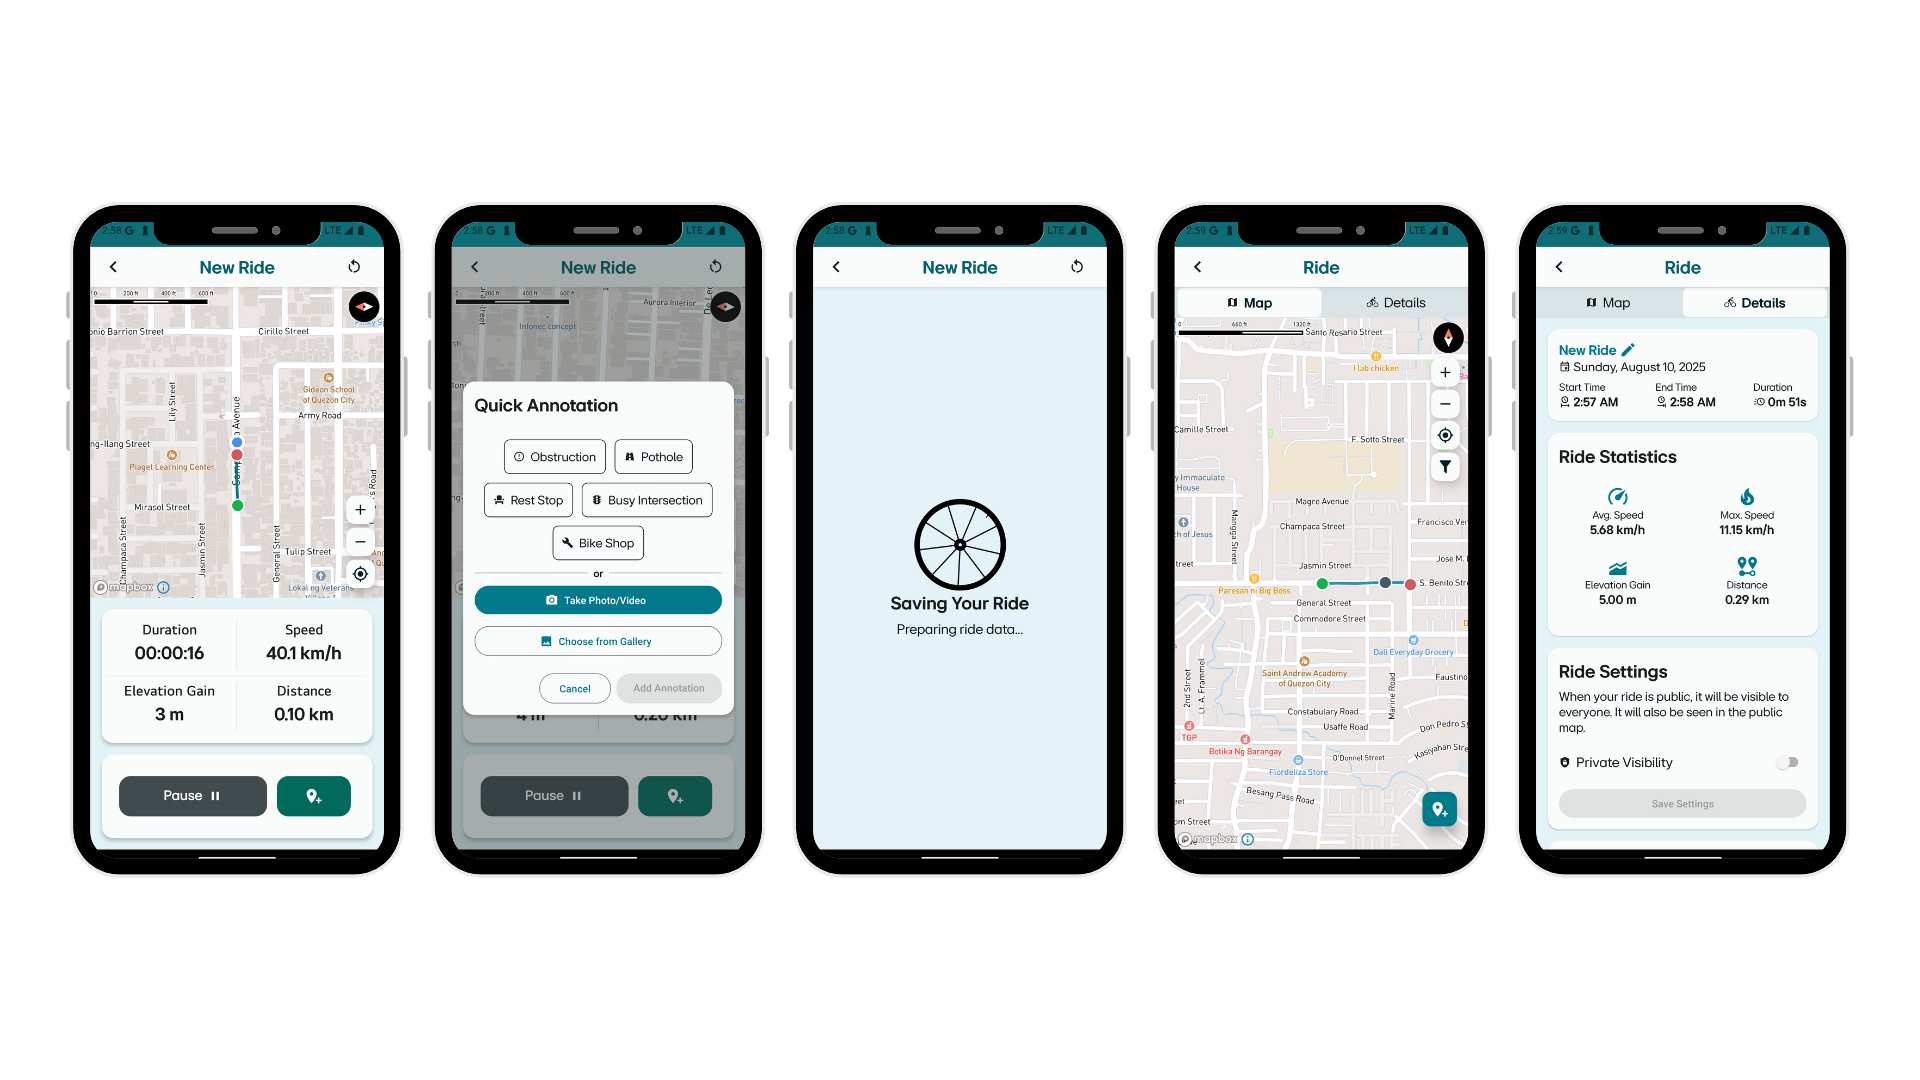
\includegraphics[width=1\linewidth]{figures/chapt5/core_features/RideRecording.png}
\caption{In-app screenshots of the ride recording and upload flow in WeCyclePH, showing the capture of geospatial data, real-time annotations, and the post-ride summary before secure storage in the cloud.}
\label{fig:core_riderecording}
\end{figure}


\subsection{GPX Uploads as Rides}
Alternatively, users may upload GPX files exported from third-party cycling devices. Upon upload, the file is parsed using a dedicated GPX parser library (\texttt{fast-xml-parser}). Parsed GPS points are structured into a ride document consistent with native mobile app rides. Metadata such as route name, start time, and device source are inferred and saved alongside the data.

Users may also attach annotations to these imported rides using the same mechanisms available for mobile-captured trips. As with mobile-recorded rides, each annotation includes an optional description of the user's emotional state during that segment.

\begin{figure}[H]
\centering
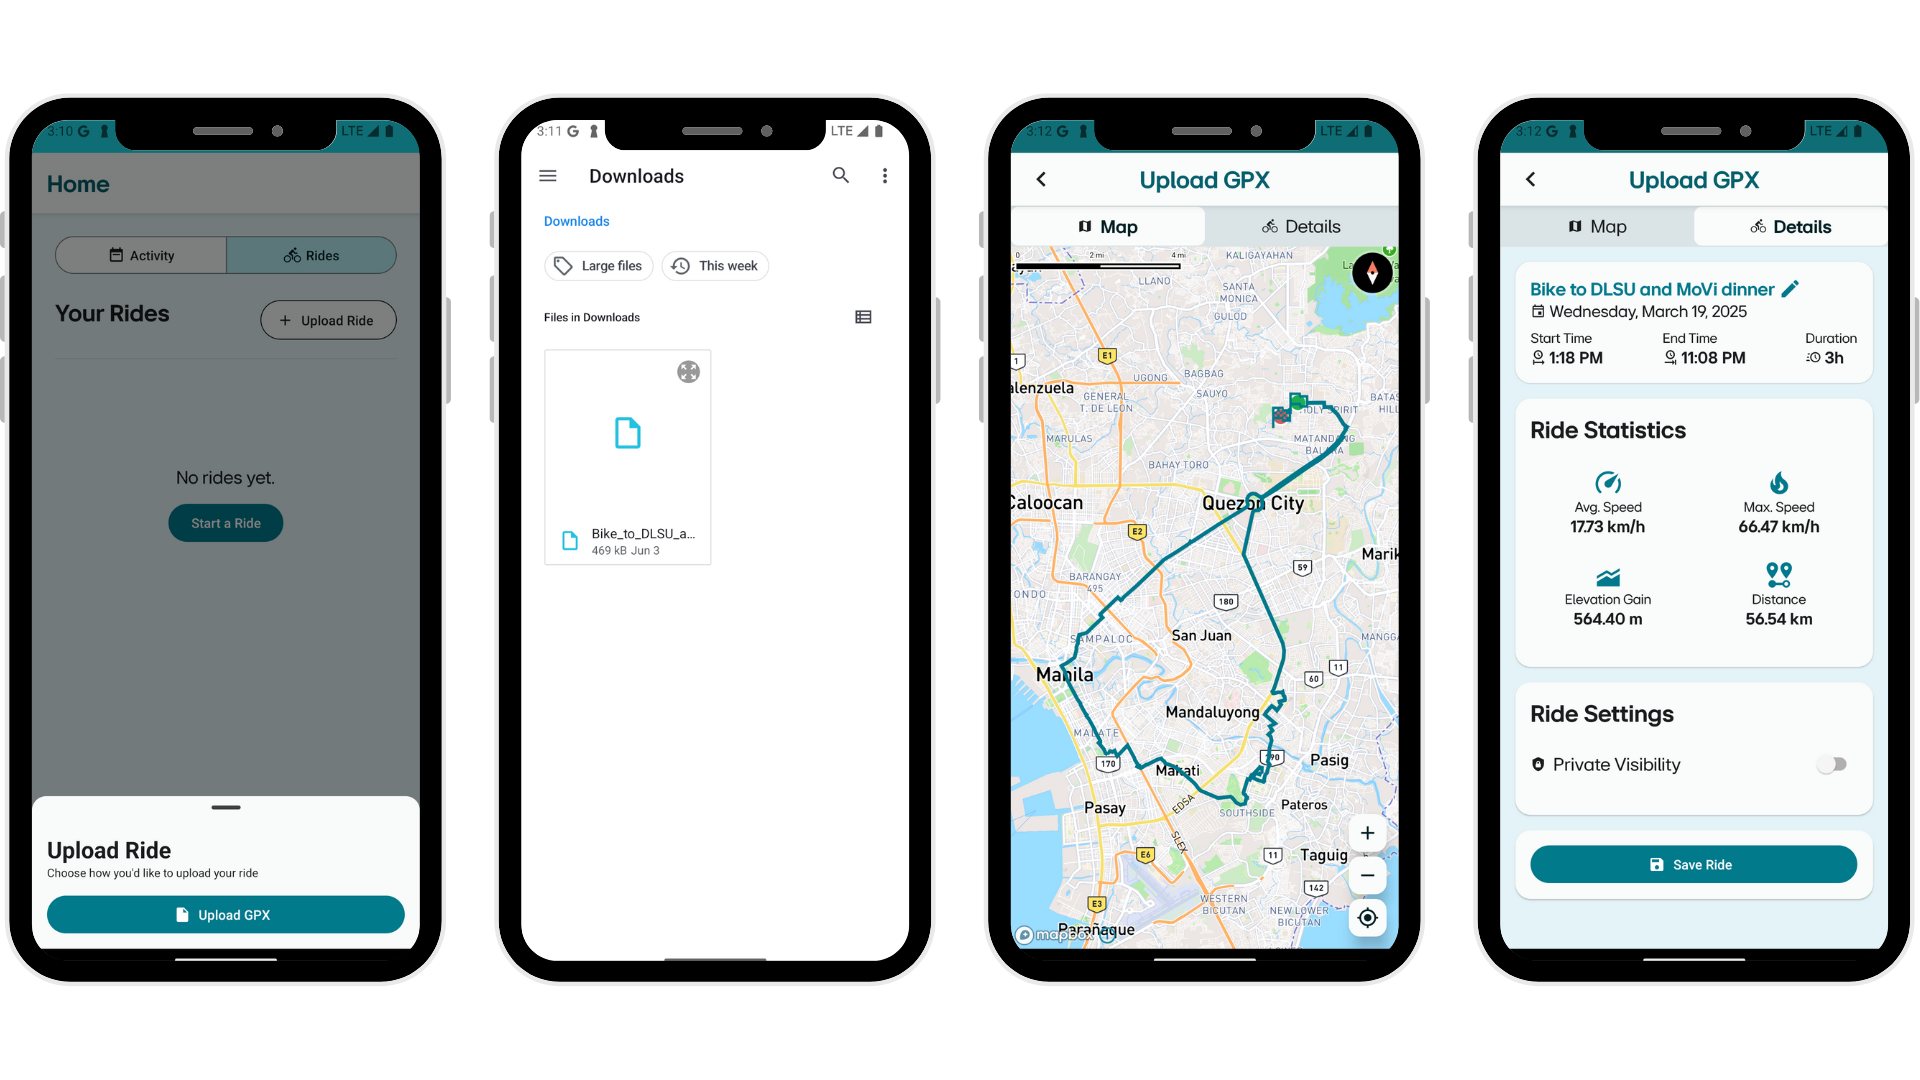
\includegraphics[width=1\linewidth]{figures/chapt5/core_features/GPXUpload.png}
\caption{In-app screenshots of the GPX ride upload process in WeCyclePH, illustrating how third-party cycling data is parsed to match the format of mobile-recorded rides.}
\label{fig:core-gpxupload}
\end{figure}

\subsection{Annotations}
The WeCyclePH platform supports the addition of rich, geolocated annotations to recorded rides, enabling cyclists to document road conditions, hazards, amenities, and personal experiences in a structured format. Annotations may be added in three ways:
\begin{itemize}
    \item During the ride via quick in-app tagging or media capture.
    \item After the ride through the mobile or web interface.
    \item Automatically, through the system's machine-learning–powered media analysis pipeline.
\end{itemize}

\subsubsection{Annotation Types}
The application supports three main annotation types, each linked to the ride via GPS coordinates and timestamp:

\begin{itemize}
\item \textbf{Point Annotations}: These annotations represent single-location events such as potholes, rest stops, or obstructions. Users can tag these during the ride or afterward by selecting a specific coordinate on the map. Timestamp and geolocation data are used to associate the annotation with the route.

\item \textbf{Segment Annotations}: These represent conditions experienced over a stretch of the ride, such as "bike lane available" or "rough surface." These can be annotated post-ride by selecting a start and end segment or are inferred automatically using detection logic applied to video frames.

\item \textbf{Media Annotations}: When users upload images or video clips, the system extracts metadata (timestamp, geolocation) if available. The backend automatically attempts to align the media to the closest matching point or segment on the ride timeline. If no metadata is present, users are prompted to manually anchor the media by selecting a position on the map or route.

\end{itemize}

Each annotation includes an optional emotional context field where users may describe their subjective experience (e.g., safe, stressed, frustrated). This qualitative layer complements objective geospatial and environmental data, providing richer interpretability.

\begin{figure}[H]
\centering
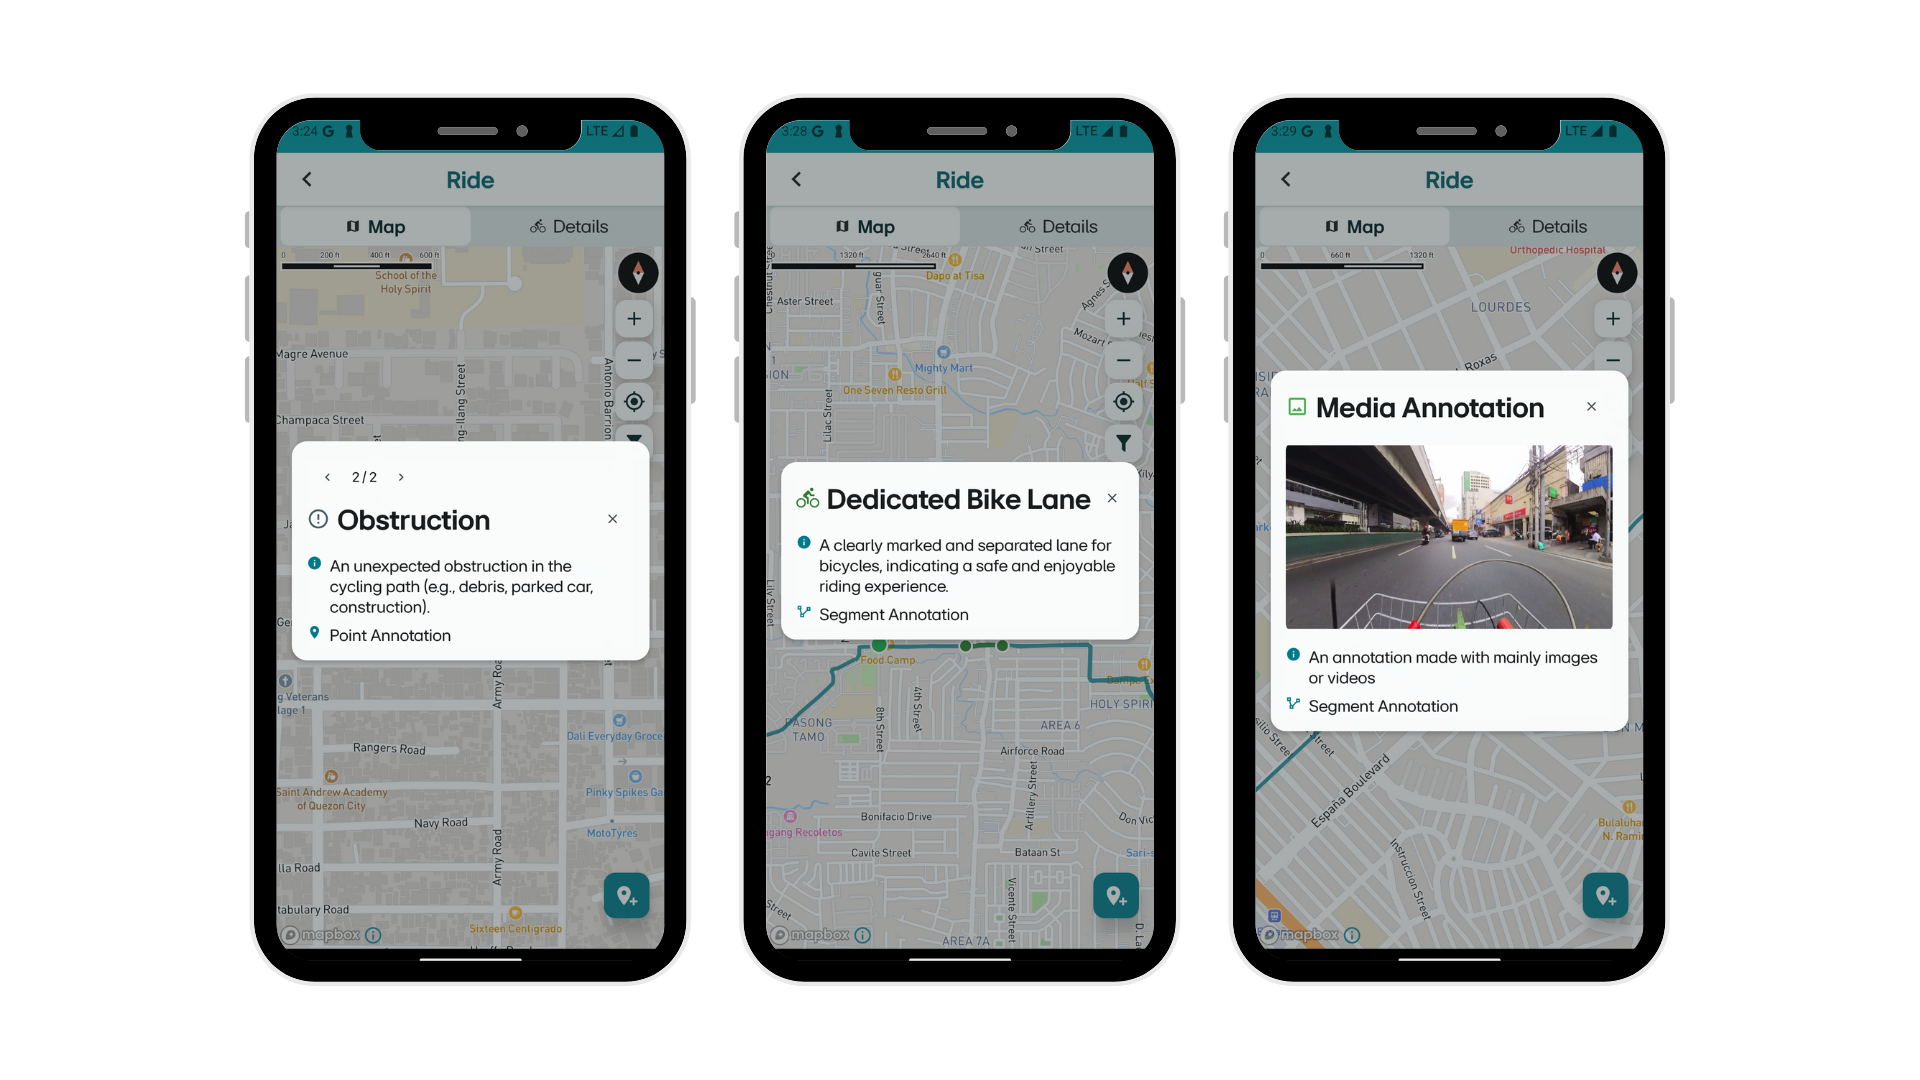
\includegraphics[width=1\linewidth]{figures/chapt5/core_features/AnnotationTypes.png}
\caption{In-app screenshots illustrating the three main annotation types in WeCyclePH: point, segment, and media—each linked to GPS coordinates and timestamps, with optional emotional context to capture cyclists’ subjective experiences alongside objective ride data.}
\label{fig:core-annotationtypes}
\end{figure}

\subsubsection{Predefined User Annotation Labels}
\label{sec:predefined-annotations}
To maintain consistency and enable comparative analysis, the system provides a fixed set of predefined labels (Table~\ref{tab:annotation_mapping}). These include infrastructure elements (Bike lane, Barrier bollard), surface conditions (Smooth surface, Pothole), traffic context (High traffic, Low traffic), and other relevant categories. All labels can be applied as point or segment annotations, and may optionally include media.

\begin{table}[H]
\centering
\begin{tabular}{|p{4.5cm}|p{2.5cm}|p{6.5cm}|}
\hline
\textbf{Annotation Label} & \textbf{Type} & \textbf{Description} \\
\hline
\texttt{Bike lane} & Segment & Indicates presence of a designated bike lane. \\
\hline
\texttt{Shared Road} & Segment & Cyclists share the road with other vehicles. \\
\hline
\texttt{No Bike Lane} & Segment & Absence of bike lanes on the road. \\
\hline
\texttt{Barrier Bollard} & Segment & Protective barriers or bollards present. \\
\hline
\texttt{Pothole} & Point & Potholes encountered. \\
\hline
\texttt{Rough Surface} & Segment & Poor or uneven road surface. \\
\hline
\texttt{Smooth Surface} & Segment & Well-maintained, smooth road conditions. \\
\hline
\texttt{Steep Incline} & Segment & Uphill segments that require extra effort. \\
\hline
\texttt{Steep Decline} & Segment & Downhill segments. \\
\hline
\texttt{Rest Stop} & Point & Areas where cyclists may safely rest. \\
\hline
\texttt{Construction} & Point & Ongoing roadworks or construction zones. \\
\hline
\texttt{Intersection} & Point & Major intersections or junctions. \\
\hline
\texttt{Bike Shop} & Point & Proximity to a bike shop. \\
\hline
\texttt{High Traffic} & Segment & Areas with heavy vehicular traffic. \\
\hline
\texttt{Low Traffic} & Segment & Segments with minimal vehicular traffic. \\
\hline
\texttt{Media Annotation} & Point/Segment & Annotation paired with an image or video. \\
\hline
\end{tabular}
\caption{Predefined user annotation labels in WeCyclePH, covering infrastructure, surface conditions, traffic context, and other cycling-relevant categories, ensuring consistent tagging for both point and segment annotations with optional media attachments.}
\label{tab:annotation_mapping}
\end{table}

\subsubsection{Manual Annotation Workflow}
Users can annotate during a ride by tapping the live map to place a marker, selecting a label, and optionally attaching media. Post-ride, the ride history view allows adding new annotations, adjusting segment boundaries, or editing/deleting existing entries. The interface supports drawing segments for continuous conditions and pinpointing discrete issues, ensuring flexibility in representing the cycling experience.

\begin{figure}[H]
\centering
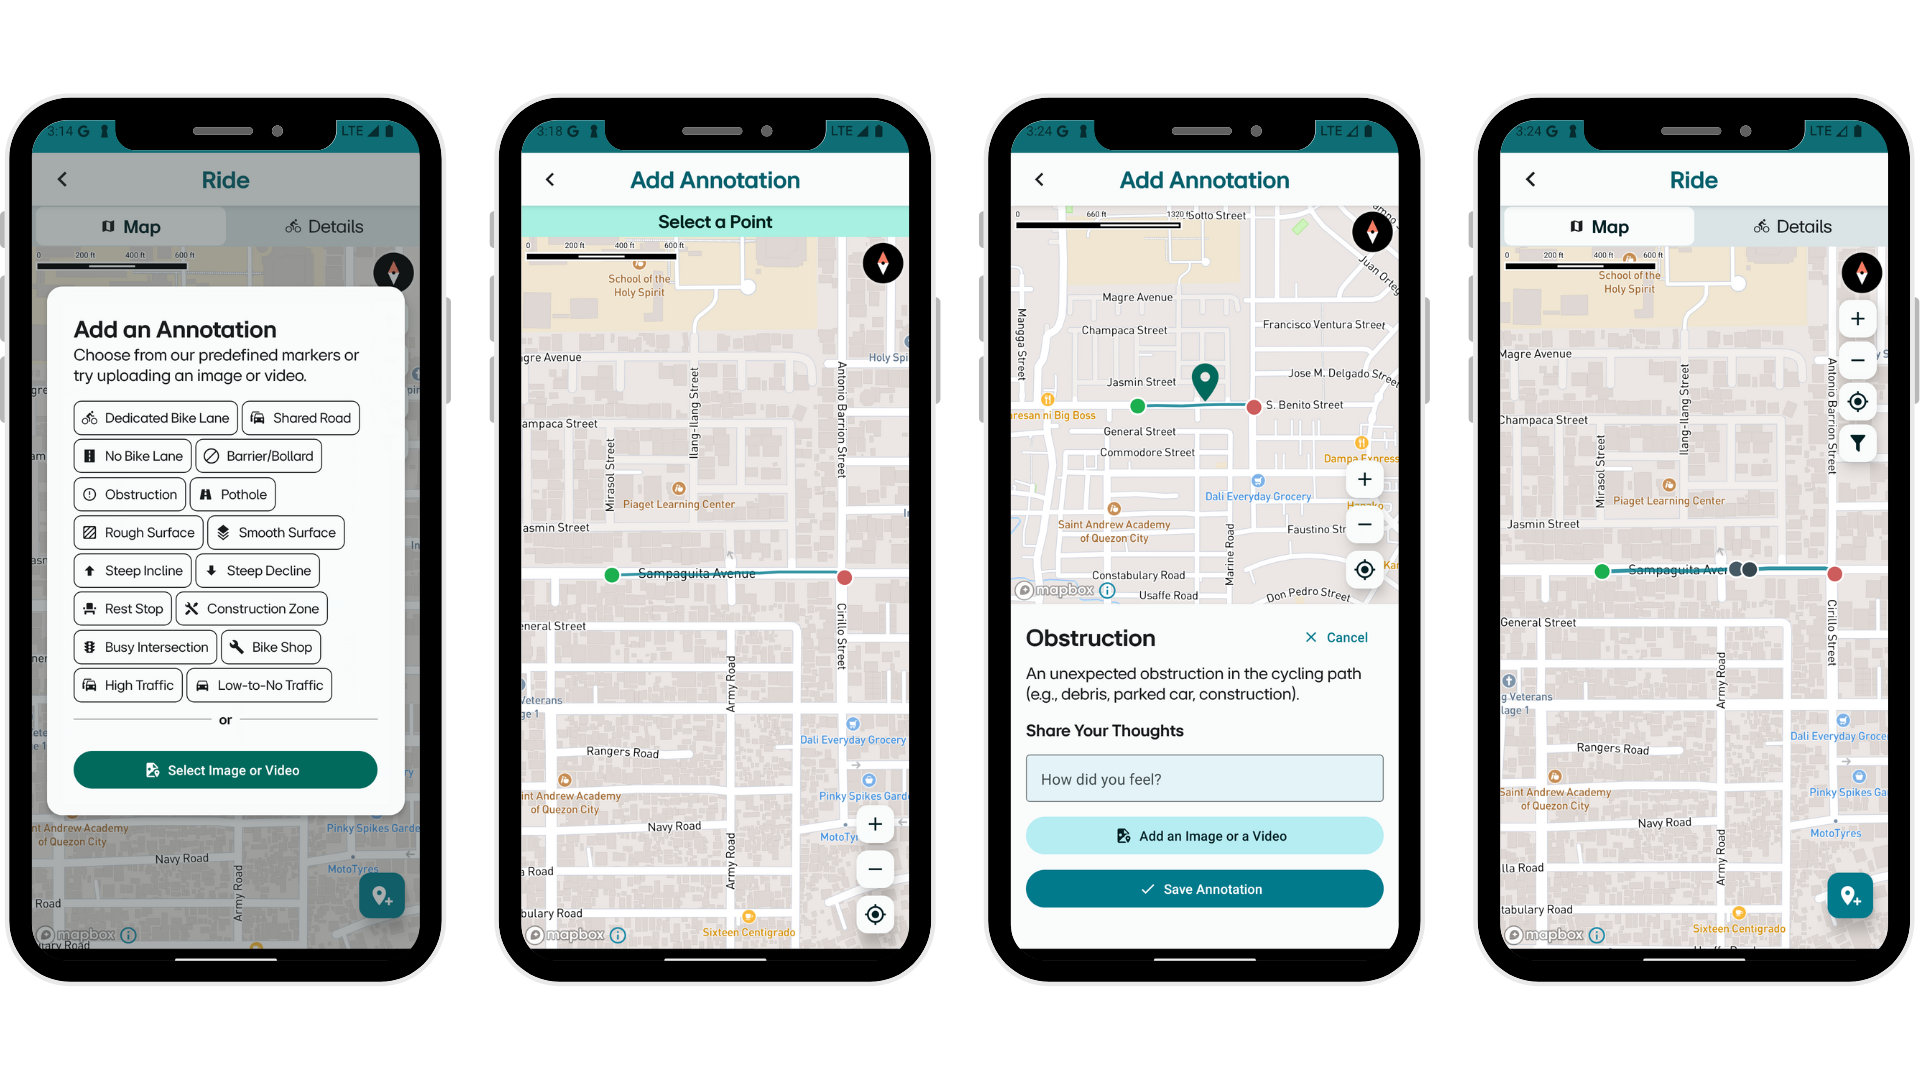
\includegraphics[width=1\linewidth]{figures/chapt5/core_features/ManualAnnotations.png}
\caption{In-app screenshots of the manual annotation workflow in WeCyclePH, showing how users can add point or segment annotations during or after a ride, select predefined labels, attach media, and edit or adjust entries to accurately represent their cycling experience.}
\label{fig:core-manualannotation}
\end{figure}

\subsubsection{Automated Annotation via Media Inference}

While the WeCyclePH mobile application supports user uploads of media such as videos and images, the annotation inference process is not conducted within the mobile app due to computational constraints. Instead, a separate, locally run processing tool handles the generation of annotations through an external instance segmentation API.

Uploaded media are first downloaded from Firebase Cloud Storage and parsed locally by a custom script. This script extracts frames at regular intervals and submits them to a fine-tuned YOLOv11 instance segmentation model hosted via an inference API. Detected objects—including \texttt{bike lanes}, \texttt{potholes}, \texttt{barriers}, and various vehicle types—are processed into annotations using rule-based logic. These are then formatted to match the WeCyclePH annotation schema.

Once the inference process is complete, the resulting annotations are uploaded back into the Firebase backend and appear alongside user-generated annotations for visualization and analysis. While these machine-generated annotations are not yet editable in-app, they enrich the dataset by identifying features users may have missed and supporting consistent tagging across rides.

This semi-automated approach allows the platform to augment user-submitted data without requiring on-device inference, preserving both mobile performance and annotation consistency.
